% Created 2011-05-18 Wed 15:15
\documentclass[presentation]{beamer}
\usepackage[latin1]{inputenc}
\usepackage[T1]{fontenc}
\usepackage{fixltx2e}
\usepackage{graphicx}
\usepackage{longtable}
\usepackage{float}
\usepackage{wrapfig}
\usepackage{soul}
\usepackage{textcomp}
\usepackage{marvosym}
\usepackage{wasysym}
\usepackage{latexsym}
\usepackage{amssymb}
\usepackage{hyperref}
\tolerance=1000
\usepackage[english]{babel} \usepackage{ae,aecompl}
\usepackage{mathpazo,courier,euler} \usepackage[scaled=.95]{helvet}
\usepackage{listings}
\lstset{language=Python, basicstyle=\ttfamily\bfseries,
commentstyle=\color{red}\itshape, stringstyle=\color{darkgreen},
showstringspaces=false, keywordstyle=\color{blue}\bfseries}
\providecommand{\alert}[1]{\textbf{#1}}

\title{}
\author{FOSSEE}
\date{}

\usetheme{Warsaw}\usecolortheme{default}\useoutertheme{infolines}\setbeamercovered{transparent}
\begin{document}











\begin{frame}

\begin{center}
\vspace{12pt}
\textcolor{blue}{\huge Using Plot Interactively}
\end{center}
\vspace{18pt}
\begin{center}
\vspace{10pt}

\includegraphics[scale=0.95]{../images/fossee-logo.png}\\
\vspace{5pt}
\scriptsize Developed by FOSSEE Team, IIT-Bombay. \\ 
\scriptsize Funded by National Mission on Education through ICT\\
\scriptsize  MHRD,Govt. of India\\

\includegraphics[scale=0.30]{../images/iitb-logo.png}\\
\end{center}
\end{frame}
\begin{frame}
\frametitle{Objectives}
\label{sec-2}

  At the end of this tutorial, you will be able to, 

\begin{itemize}
\item Create simple plots of mathematical functions.
\item Use the Figure window to study plots better.
\end{itemize}
\end{frame}
\begin{frame}
\frametitle{Error if Ipython not installed}
\label{sec-3}
\begin{itemize}

\item `ERROR: matplotlib could NOT be imported!  Starting normal IPython.`\\
\label{sec-3_1}%
\end{itemize} % ends low level
\end{frame}
\begin{frame}
\frametitle{Plot UI}
\label{sec-4}

   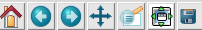
\includegraphics[height=0.12in, interpolate=true]{buttons}

\begin{itemize}
\item Save
\item Zoom
\item Move axis
\item Back and Forward Button
\item Home
\end{itemize}
\end{frame}
\begin{frame}
\frametitle{Question 1}
\label{sec-5}

  Plot (sin(x)*sin(x))/x.

\begin{enumerate}
\item Save the plot by the sinsquarebyx.pdf in pdf format.
\item Zoom and find the maxima.
\item Bring it back to initial position.
\end{enumerate}
\end{frame}
\begin{frame}
\frametitle{Summary}
\label{sec-6}

  In this tutorial,we have learnt to-

\begin{itemize}
\item Start Ipython with pylab.
\item Use the linspace function to create `num` equally spaced points in a region.
\item Find the length of sequnces using len function.
\item Plot mathematical functions using plot.
\item Clear drawing area using clf.
\item Plott mathematical functions using plot.
\item Use the UI of plot
\begin{itemize}
\item Save
\item Zoom
\item Move axis
\item Back and Forward Button
\item Home
\end{itemize}
\end{itemize}
 
\end{frame}
\begin{frame}
\frametitle{Evaluation}
\label{sec-7}


\begin{enumerate}
\item Create 100 equally spaced points between -pi/2 and pi/2?
\item What will the command `'linspace(-pi,pi,100)'' do.
\begin{itemize}
\item returns 100 evenly spaced samples from -pi to pi
\item returns 100 evenly spaced samples from -pi to pi excluding pi but including -pi
\item returns 100 evenly spaced samples from -pi to pi excluding -pi but including pi
\item returns 100 evenly spaced samples from -pi to pi including both -pi and pi
\end{itemize}
\item How do find the length of a sequence.
\end{enumerate}
\end{frame}
\begin{frame}
\frametitle{Solutions\ldots{}}
\label{sec-8}


\begin{enumerate}
\item linspace(-pi/2,pi/2,100)
\item returns 100 evenly spaced samples from -pi to pi including both -pi and pi
\item len(sequence\_name)
\end{enumerate}
\end{frame}
\begin{frame}

 \begin{block}{}
  \begin{center}
  \textcolor{blue}{\Large THANK YOU!} 
  \end{center}
  \end{block}
\begin{block}{}
  \begin{center}
    For more Information, visit our website\\
    \url{http://fossee.in/}
  \end{center}  
  \end{block}
\end{frame}

\end{document}